%%%%%%%%%%%%%%%%%%%%%%
%% Document details %%
%%%%%%%%%%%%%%%%%%%%%%

% Paper title
\title{SkelCL Initial Performance Results}

% Author
\author{Chris Cummins}

%%%%%%%%%%%%%%%%%%%%%%%%%
%% Document and Layout %%
%%%%%%%%%%%%%%%%%%%%%%%%%

% Fix for multiple "No room for a new \dimen" errors.
%
% See: http://tex.stackexchange.com/questions/38607/no-room-for-a-new-dimen
%
\usepackage{etex}

\usepackage{booktabs}

\usepackage[utf8]{inputenc}

% Make internal macro definitions accessible,
% e.g. \@title, \@date \@author.
\makeatletter

% Multi-column support.
\usepackage{multicol}

% A useful package which includes macros like \ifdef{}{}{}:
%
\usepackage{etoolbox}

% Uncomment the following line to remove column separation:
%
%\setlength{\columnsep}{5mm}


% Set chapter and section numbering depth:
%
\setcounter{secnumdepth}{2}


%%%%%%%%%%%%%%%%%%%%%%%%%%%%%%%%%
%% Bibliography and Appendices %%
%%%%%%%%%%%%%%%%%%%%%%%%%%%%%%%%%
\usepackage[%
    backend=biber,
    style=numeric-comp,  % numerical-compressed
    sorting=none,        % nty,nyt,nyvt,anyt,anyvt,ynt,ydnt,none
    sortcites=true,      % sort \cite{b a d c}: true,false
    block=none,          % space between blocks: none,space,par,nbpar,ragged
    indexing=false,      % indexing options: true,false,cite,bib
    citereset=none,      % don't reset cites
    isbn=false,          % print ISBN?
    url=false,           % print URL?
    doi=false,           % print DOI?
    natbib=true,         % natbib compatability
  ]{biblatex}

% Reduce the font size of the bibliography:
% \renewcommand{\bibfont}{\normalfont\scriptsize}

% Determine which BibTeX file to use:
%
% If available, use my Mendeley BibTex library, located in the home
% directory. Note that this is a relative path and will break if
% either this file or the BibTex library are moved. If the library is
% not present, use the local refs.bib file.
\newcommand{\BibResourceGlobal}{../../../../library.bib}
\newcommand{\BibResourceLocal}{refs.bib}

\IfFileExists{\BibResourceGlobal}
  {\newcommand{\BibResource}{\BibResourceGlobal}}
  {\newcommand{\BibResource}{\BibResourceLocal}}

\addbibresource{\BibResource}

% Appendix package. Documentation:
%
%  http://mirror.ox.ac.uk/sites/ctan.org/macros/latex/contrib/appendix/appendix.pdf
%
% Package options:
%
% toc      - Put a header (e.g., `Appendices') into the Table of Contents
%            (the ToC) before listing the appendices. (This is done by
%            calling the \addappheadtotoc command.)
% page     - Puts a title (e.g., `Appendices') into the document at the
%            point where the appendices environment is begun. (This is
%            done by calling the \appendixpage command.)
% title    - Adds a name (e.g., `Appendix') before each appendix title in
%            the body of the document. The name is given by the value
%            of \appendixname. Note that this is the default behaviour
%            for classes that have chapters.
% titletoc - Adds a name (e.g., `Appendix') before each appendix listed
%            in the ToC. The name is given by the value
%            of \appendixname.
% header   - Adds a name (e.g., `Appendix') before each appendix in page
%            headers.  The name is given by the value
%            of \appendixname. Note that this is the default behaviour
%            for classes that have chapters.
\usepackage[title, titletoc]{appendix}


%%%%%%%%%%%%%%%%%%%%%%%%%%%%%%%%%%%%%
%% Figures, footnotes and listings %%
%%%%%%%%%%%%%%%%%%%%%%%%%%%%%%%%%%%%%

%\usepackage{float}
%\restylefloat{figure}

% Use bold ``(Figure|Table|Listing)'' caption text.
%\usepackage[margin=1cm]{caption}

% Set the font for captions.
%\renewcommand{\captionfont}{\footnotesize}
% Set the font for caption labels.
%\renewcommand{\captionlabelfont}{\footnotesize\bf}

% Use arabic numbers for footnote.
%\renewcommand{\thefootnote}{\arabic{footnote}}

% Ensure that footnotes always appear at the bottom of pages.
%\usepackage[bottom]{footmisc}

% Reset the footnote counter on every page.
%\usepackage{perpage}
%\MakePerPage{footnote}

% Pre-requisites for rendering upquotes in listings package.
\usepackage[T1]{fontenc}
\usepackage{lmodern}
\usepackage{textcomp}

% Pseudo-code listings.
\usepackage{algorithm}
\usepackage{algpseudocode}
\newcommand{\Break}{\State \textbf{break} }
\algblockdefx[Loop]{Loop}{EndLoop}[1][]{\textbf{Loop} #1}{\textbf{End
    Loop}}

\algrenewcommand\ALG@beginalgorithmic{\footnotesize}

% Code listings.
\usepackage{listings}

% Set \ttfamily to use courier fonts.
%
% See: http://tex.stackexchange.com/a/33686
%
\usepackage{courier}

\lstset{frame=bt,                    % Add top and bottom frame lines
        breaklines=true,             % Force line wrapping
        captionpos=b,                % Place caption below listing
        numbers=left,                % Add left-side line numbers
        basicstyle=\scriptsize\ttfamily, % Set font size and type
        showstringspaces=false,      % Don't show visible whitespace
        numberstyle=\tiny,
        upquote=true,                % Use upright quotes, not curly
        commentstyle=\bfseries}      % Embolden comments

% Use (*@ @*) to escape LaTeX commands within listings.
\lstset{escapeinside={(*@}{@*)}}

% Add 10pt space between chapters in TOC listings entries:
%\let\Chapter\chapter
%\def\chapter{\addtocontents{lol}{\protect\addvspace{10pt}}\Chapter}

% Add JavaScript support to listings. See:
%
%     http://tex.stackexchange.com/a/89576
%
\lstdefinelanguage{JavaScript}{
  keywords={
    break,
    case,
    catch,
    catch,
    do,
    else,
    false,
    function,
    if,
    in,
    new,
    null,
    return,
    switch,
    true,
    typeof,
    var,
    while}
  keywordstyle=\bfseries,
  ndkeywords={
    boolean,
    class,
    export,
    implements,
    import,
    this,
    throw}
  ndkeywordstyle=\bfseries,
  sensitive=false,
  comment=[l]{//},
  morecomment=[s]{/*}{*/},
  morestring=[b]',
  morestring=[b]"
}

% Add Clojure support to listings. See:
%
%     http://alexott.blogspot.co.uk/2010/01/clojure-latex.html
%
\lstdefinelanguage{Clojure}{morekeywords={
    *,
    *1,
    *2,
    *3,
    *agent*,
    *allow-unresolved-vars*,
    *assert*,
    *clojure-version*,
    *command-line-args*,
    *compile-files*,
    *compile-path*,
    *e,
    *err*,
    *file*,
    *flush-on-newline*,
    *in*,
    *macro-meta*,
    *math-context*,
    *ns*,
    *out*,
    *print-dup*,
    *print-length*,
    *print-level*,
    *print-meta*,
    *print-readably*,
    *read-eval*,
    *source-path*,
    *use-context-classloader*,
    *warn-on-reflection*,
    +,
    -,
    ->,
    ->>,
    ..,
    /,
    :else,
    <,
    <=,
    =,
    ==,
    >,
    >=,
    @,
    accessor,
    aclone,
    add-classpath,
    add-watch,
    agent,
    agent-errors,
    aget,
    alength,
    alias,
    all-ns,
    alter,
    alter-meta!,
    alter-var-root,
    amap,
    ancestors,
    and,
    apply,
    areduce,
    array-map,
    aset,
    aset-boolean,
    aset-byte,
    aset-char,
    aset-double,
    aset-float,
    aset-int,
    aset-long,
    aset-short,
    assert,
    assoc,
    assoc!,
    assoc-in,
    associative?,
    atom,
    await,
    await-for,
    await1,
    bases,
    bean,
    bigdec,
    bigint,
    binding,
    bit-and,
    bit-and-not,
    bit-clear,
    bit-flip,
    bit-not,
    bit-or,
    bit-set,
    bit-shift-left,
    bit-shift-right,
    bit-test,
    bit-xor,
    boolean,
    boolean-array,
    booleans,
    bound-fn,
    bound-fn*,
    butlast,
    byte,
    byte-array,
    bytes,
    cast,
    char,
    char-array,
    char-escape-string,
    char-name-string,
    char?,
    chars,
    chunk,
    chunk-append,
    chunk-buffer,
    chunk-cons,
    chunk-first,
    chunk-next,
    chunk-rest,
    chunked-seq?,
    class,
    class?,
    clear-agent-errors,
    clojure-version,
    coll?,
    comment,
    commute,
    comp,
    comparator,
    compare,
    compare-and-set!,
    compile,
    complement,
    concat,
    cond,
    condp,
    conj,
    conj!,
    cons,
    constantly,
    construct-proxy,
    contains?,
    count,
    counted?,
    create-ns,
    create-struct,
    cycle,
    dec,
    decimal?,
    declare,
    def,
    definline,
    defmacro,
    defmethod,
    defmulti,
    defn,
    defn-,
    defonce,
    defprotocol,
    defstruct,
    deftype,
    delay,
    delay?,
    deliver,
    deref,
    derive,
    descendants,
    destructure,
    disj,
    disj!,
    dissoc,
    dissoc!,
    distinct,
    distinct?,
    do,
    do-template,
    doall,
    doc,
    dorun,
    doseq,
    dosync,
    dotimes,
    doto,
    double,
    double-array,
    doubles,
    drop,
    drop-last,
    drop-while,
    empty,
    empty?,
    ensure,
    enumeration-seq,
    eval,
    even?,
    every?,
    false,
    false?,
    ffirst,
    file-seq,
    filter,
    finally,
    find,
    find-doc,
    find-ns,
    find-var,
    first,
    float,
    float-array,
    float?,
    floats,
    flush,
    fn,
    fn?,
    fnext,
    for,
    force,
    format,
    future,
    future-call,
    future-cancel,
    future-cancelled?,
    future-done?,
    future?,
    gen-class,
    gen-interface,
    gensym,
    get,
    get-in,
    get-method,
    get-proxy-class,
    get-thread-bindings,
    get-validator,
    hash,
    hash-map,
    hash-set,
    identical?,
    identity,
    if,
    if-let,
    if-not,
    ifn?,
    import,
    in-ns,
    inc,
    init-proxy,
    instance?,
    int,
    int-array,
    integer?,
    interleave,
    intern,
    interpose,
    into,
    into-array,
    ints,
    io!,
    isa?,
    iterate,
    iterator-seq,
    juxt,
    key,
    keys,
    keyword,
    keyword?,
    last,
    lazy-cat,
    lazy-seq,
    let,
    letfn,
    line-seq,
    list,
    list*,
    list?,
    load,
    load-file,
    load-reader,
    load-string,
    loaded-libs,
    locking,
    long,
    long-array,
    longs,
    loop,
    macroexpand,
    macroexpand-1,
    make-array,
    make-hierarchy,
    map,
    map?,
    mapcat,
    max,
    max-key,
    memfn,
    memoize,
    merge,
    merge-with,
    meta,
    method-sig,
    methods,
    min,
    min-key,
    mod,
    monitor-enter,
    monitor-exit,
    name,
    namespace,
    neg?,
    new,
    newline,
    next,
    nfirst,
    nil,
    nil?,
    nnext,
    not,
    not-any?,
    not-empty,
    not-every?,
    not=,
    ns,
    ns-aliases,
    ns-imports,
    ns-interns,
    ns-map,
    ns-name,
    ns-publics,
    ns-refers,
    ns-resolve,
    ns-unalias,
    ns-unmap,
    nth,
    nthnext,
    num,
    number?,
    odd?,
    or,
    parents,
    partial,
    partition,
    pcalls,
    peek,
    persistent!,
    pmap,
    pop,
    pop!,
    pop-thread-bindings,
    pos?,
    pr,
    pr-str,
    prefer-method,
    prefers,
    primitives-classnames,
    print,
    print-ctor,
    print-doc,
    print-dup,
    print-method,
    print-namespace-doc,
    print-simple,
    print-special-doc,
    print-str,
    printf,
    println,
    println-str,
    prn,
    prn-str,
    promise,
    proxy,
    proxy-call-with-super,
    proxy-mappings,
    proxy-name,
    proxy-super,
    push-thread-bindings,
    pvalues,
    quot,
    rand,
    rand-int,
    range,
    ratio?,
    rational?,
    rationalize,
    re-find,
    re-groups,
    re-matcher,
    re-matches,
    re-pattern,
    re-seq,
    read,
    read-line,
    read-string,
    recur,
    reduce,
    ref,
    ref-history-count,
    ref-max-history,
    ref-min-history,
    ref-set,
    refer,
    refer-clojure,
    reify,
    release-pending-sends,
    rem,
    remove,
    remove-method,
    remove-ns,
    remove-watch,
    repeat,
    repeatedly,
    replace,
    replicate,
    require,
    reset!,
    reset-meta!,
    resolve,
    rest,
    resultset-seq,
    reverse,
    reversible?,
    rseq,
    rsubseq,
    second,
    select-keys,
    send,
    send-off,
    seq,
    seq?,
    seque,
    sequence,
    sequential?,
    set,
    set!,
    set-validator!,
    set?,
    short,
    short-array,
    shorts,
    shutdown-agents,
    slurp,
    some,
    sort,
    sort-by,
    sorted-map,
    sorted-map-by,
    sorted-set,
    sorted-set-by,
    sorted?,
    special-form-anchor,
    special-symbol?,
    split-at,
    split-with,
    str,
    stream?,
    string?,
    struct,
    struct-map,
    subs,
    subseq,
    subvec,
    supers,
    swap!,
    symbol,
    symbol?,
    sync,
    syntax-symbol-anchor,
    take,
    take-last,
    take-nth,
    take-while,
    test,
    the-ns,
    throw,
    time,
    to-array,
    to-array-2d,
    trampoline,
    transient,
    tree-seq,
    true,
    true?,
    try,
    type,
    unchecked-add,
    unchecked-dec,
    unchecked-divide,
    unchecked-inc,
    unchecked-multiply,
    unchecked-negate,
    unchecked-remainder,
    unchecked-subtract,
    underive,
    unquote,
    unquote-splicing,
    update-in,
    update-proxy,
    use,
    val,
    vals,
    var,
    var-get,
    var-set,
    var?,
    vary-meta,
    vec,
    vector,
    vector?,
    when,
    when-first,
    when-let,
    when-not,
    while,
    with-bindings,
    with-bindings*,
    with-in-str,
    with-loading-context,
    with-local-vars,
    with-meta,
    with-open,
    with-out-str,
    with-precision,
    xml-seq,
    zero?,
    zipmap
  },
  sensitive,
  alsodigit=-,
  morecomment=[l];,
  morestring=[b]"
}[keywords,comments,strings]


%%%%%%%%%%%%%%%%%%%%%%%%
%% Graphics and maths %%
%%%%%%%%%%%%%%%%%%%%%%%%
\usepackage{amsmath}

% Additional amsmath symbols, see:
%
% http://texblog.org/2007/08/27/number-sets-prime-natural-integer-rational-real-and-complex-in-latex/
%
\usepackage{amssymb}

\usepackage{graphicx}
\usepackage{mathtools}
\usepackage{tikz}
\usepackage{tikz-qtree}

% Provide bold font face in maths.
\usepackage{bm}

\usepackage{subcaption}
\expandafter\def\csname ver@subfig.sty\endcsname{}

% Define an 'myalignat' command which behave as 'alignat' without the
% vertical top and bottom padding. See:
%     http://www.latex-community.org/forum/viewtopic.php?f=5&t=1890
\newenvironment{myalignat}[1]{%
  \setlength{\abovedisplayskip}{-.7\baselineskip}%
  \setlength{\abovedisplayshortskip}{\abovedisplayskip}%
  \start@align\z@\st@rredtrue#1
}%
{\endalign}

% Define additional operators:
\DeclareMathOperator*{\argmin}{arg\,min}
\DeclareMathOperator*{\argmax}{arg\,max}

% Skeleton operators.
\DeclareMathOperator*{\map}{Map}
\DeclareMathOperator*{\reduce}{Reduce}
\DeclareMathOperator*{\scan}{Scan}
\DeclareMathOperator*{\stencil}{Stencil}
\DeclareMathOperator*{\zip}{Zip}
\DeclareMathOperator*{\allpairs}{All\,Pairs}

% Maths plots using pgfplots, see:
%
%     http://pgfplots.sourceforge.net/pgfplots.pdf
%
\usepackage{pgfplots}

% Gantt charts using pgfgantt, see:
%
%     http://www.ctan.org/pkg/pgfgantt
%
\usepackage{pgfgantt}

% Fix milestone aspect ratio by defining a custom element.
\newganttchartelement*{mymilestone}{
  mymilestone/.style={
    shape=diamond,
    inner sep=2pt,
    draw=black,
    top color=black,
    bottom color=black,
  }
}

% Tikz flowchart configuration.
\usetikzlibrary{shapes,arrows,shadows,fit,backgrounds}
\tikzstyle{decision} = [diamond,
                        draw,
                        text width=4.5em,
                        text badly centered,
                        node distance=3cm,
                        inner sep=0pt]
\tikzstyle{block}    = [rectangle,
                        draw,
                        text width=5em,
                        text centered,
                        node distance=3cm,
                        minimum height=4em,
                        inner sep=.2cm]
\tikzstyle{line}     = [draw, -latex']

% Add dirtree picture style, see:
%
%     http://tex.stackexchange.com/a/34268
%
\newcount\dirtree@lvl
\newcount\dirtree@plvl
\newcount\dirtree@clvl
\def\dirtree@growth{%
  \ifnum\tikznumberofcurrentchild=1\relax
    \global\advance\dirtree@plvl by 1
    \expandafter\xdef\csname dirtree@p@\the\dirtree@plvl\endcsname{\the\dirtree@lvl}
  \fi
  \global\advance\dirtree@lvl by 1\relax
  \dirtree@clvl=\dirtree@lvl
  \advance\dirtree@clvl by -\csname dirtree@p@\the\dirtree@plvl\endcsname
  \pgf@xa=0.33cm\relax
  \pgf@ya=-\baselineskip\relax
  \pgf@ya=\dirtree@clvl\pgf@ya
  \pgftransformshift{\pgfqpoint{\the\pgf@xa}{\the\pgf@ya}}%
  \ifnum\tikznumberofcurrentchild=\tikznumberofchildren
    \global\advance\dirtree@plvl by -1
  \fi
}
\tikzset{
  dirtree/.style={
    growth function=\dirtree@growth,
    every node/.style={anchor=north},
    every child node/.style={anchor=west},
    edge from parent path={(\tikzparentnode\tikzparentanchor) |- (\tikzchildnode\tikzchildanchor)}
  }
}

% UML sequence diagram macros, see:
%
%     https://code.google.com/p/pgf-umlsd/
%
% Options:
%
%     underline - Underline object names
%
\usepackage[underline=false]{pgf-umlsd}

% Support for SVG graphics.
%
% NOTE that you must pass the "--shell-escape" argument to pdflatex to
% compile. NOTE also that images *MUST* be placed within the graphics
% path.
\usepackage{svg}
\graphicspath{{img/}}

%%%%%%%%%%%%%%%%%%%%%%
%% Tables and lists %%
%%%%%%%%%%%%%%%%%%%%%%

%\usepackage{enumitem}
%\setenumerate{itemsep=0pt}

% Use no left margin for lists:
%\setlist{leftmargin=*}

\usepackage{longtable}

% Define column types L, C, R with known text justification and fixed
% widths:
\usepackage{array}
\newcolumntype{L}[1]{>{\raggedright\let\newline\\\arraybackslash\hspace{0pt}}m{#1}}
\newcolumntype{C}[1]{>{\centering\let\newline\\\arraybackslash\hspace{0pt}}m{#1}}
\newcolumntype{R}[1]{>{\raggedleft\let\newline\\\arraybackslash\hspace{0pt}}m{#1}}


%%%%%%%%%%%%%%%%%%%%%%%%%%%%%
%% Typesetting and symbols %%
%%%%%%%%%%%%%%%%%%%%%%%%%%%%%

% Adjustable font sizes in \Verbatim{}
\usepackage{fancyvrb}

%\usepackage{titlesec}
% Set section and paragraph heading fonts:
%\titleformat*{\section}{\Large\bfseries}
%\titleformat*{\subsection}{\normalsize\bfseries}
%\titleformat*{\subsubsection}{\normalsize}
%\titleformat*{\paragraph}{\large\bfseries}
%\titleformat*{\subparagraph}{\large\bfseries}

% Set section heading margins. Usage:
% \titlespacing*{<command>}{<left>}{<before>}{<after>}
%\titlespacing*{\section}{0pt}{.6em}{.3em}
%\titlespacing*{\subsection}{0pt}{.6em}{.2em}

% Set paragraph indentation size. Default is 15pt.
%\setlength{\parindent}{10pt}

% The line spacing can be globally set using \linespread:
%
% \linespread{1.2}

% Add a command \hr{} which will draw a horizontal rule the width of
% the text.
%
\newcommand{\hr}{\noindent\makebox[\linewidth]{\rule{\textwidth}{0.2pt}}}

% Add a command \br{} which will create a horizontal space of exactly
% one line height.
%
\newcommand{\br}{\hspace{\baselineskip}}

% Define a command to allow word breaking.
\newcommand*\wrapletters[1]{\wr@pletters#1\@nil}
\def\wr@pletters#1#2\@nil{#1\allowbreak\if&#2&\else\wr@pletters#2\@nil\fi}

% Define a command to create centred page titles.
\newcommand{\centredtitle}[1]{
  \begin{center}
    \large
    \vspace{0.9cm}
    \textbf{#1}
  \end{center}}

% Support hyperlinks using the \hyperref, \url and \href
% macros. Usage:
%
%    \hyperref[label_name]{''link text''}
%
%    \url{<my_url>}
%
%    \href{<my_url>}{<description>}
%
\usepackage{hyperref}

% Disable colored borders of links, cross-references etc in PDF output
\hypersetup{pdfborder={0 0 0}}

% Provide generic commands \degree, \celsius, \perthousand, \micro
% and \ohm which work both in text and maths mode.
\usepackage{gensymb}

%%%%%%%%%%%%%%%%%%%%%%%%%%%%%%%%%
%% Placeholder text generation %%
%%%%%%%%%%%%%%%%%%%%%%%%%%%%%%%%%

% Use either \blindtext or \libpsum to generate placeholder text. Also
% note the macros \blinditemize, \blindenumerate, \blinddescription.
\usepackage[english]{babel}
\usepackage{blindtext}
\usepackage{lipsum}


%%%%%%%%%%
%% Body %%
%%%%%%%%%%
\begin{document}

\maketitle

\begin{abstract}
  \noindent
  This document describes a methodology for collecting performance
  data of SkelCL applications, and proposes

  experimental results from two applications show a maximum speedup of
  3.8$\times$ (average: 1.77$\times$).
\end{abstract}

\section{Profiling SKelCL programs}

To obtain accurate performance data of SkelCL applications, profiling
timers have been added which report millisecond execution times for
three host operations:

\begin{itemize}
\item \textbf{init} Measures the time spent by the
  \texttt{skelcl::init()} function, which is responsible for
  enumerating the set of available OpenCL devices and selecting one or
  more to be used. The amount of time taken depends on the type of
  OpenCL drivers and whether they are already loaded. For the purposes
  of comparing program performance, this value is ignored.

\item \textbf{build} The time spent compiling a parameterised skeleton
  into an OpenCL program for the target device. This occurs each time
  a skeleton object is instantiated. Once compiled, programs are
  cached for reuse.

\item \textbf{prep} Before executing an OpenCL program, a preparation
  stage prepares the user input and allocates output data buffers as
  required. This occurs once per skeleton call.
\end{itemize}

\noindent
Additionally, OpenCL profiling
information\footnote{\url{https://www.khronos.org/registry/cl/sdk/1.2/docs/man/xhtml/clGetEventProfilingInfo.html}}
is gathered for each type of device operation:

\begin{itemize}
\item \textbf{upload} Host $\rightarrow$ Device data transfer.
\item \textbf{run} Runtime of the parameterised skeleton and user
  code.
\item \textbf{download} Device $\rightarrow$ Host data transfer.
\end{itemize}



\begin{figure}
\centering
\includesvg[width=.8\textwidth]{img/GameOfLife-cec-c9b9bcf6c928d805a0730f1789fe205b2f39fc09-events}
\caption{%
Example profiling information.%
}
\label{fig:events}
\end{figure}

\section{Tuning iterative stencil programs}

\begin{figure}
\begin{subfigure}[t]{0.45\textwidth}
\centering
\lstset{language=C++}
\begin{lstlisting}
Matrix<int> grid(data, numcols);
Stencil<int(int)> s(
    std::ifstream{"./Stencil.cl"},
    1, 1, 1, 1, // border size
    detail::Padding::NEUTRAL, 0,
    "func", 0);


grid = s(iterations, grid);
\end{lstlisting}
\caption{}
\label{lst:gol-stencil}
\end{subfigure}
~\hspace{1.5em}
\begin{subfigure}[t]{0.45\textwidth}
\centering
\lstset{language=C++}
\begin{lstlisting}
Matrix<int> grid(data, numcols);
MapOverlap<int(int)> s(
    std::ifstream{"./MapOverlap.cl"},
    1, // border size
    detail::Padding::NEUTRAL, 0,
    "func");

for (int i = 0; i < iterations; i++)
  grid = s(grid);
\end{lstlisting}
\caption{}
\label{lst:gol-mo}
\end{subfigure}
\caption{%
  Implementing Game of Life using (\subref{lst:gol-stencil}) Stencil
  skeleton and (\subref{lst:gol-mo}) MapOverlap skeleton.%
}
\end{figure}


\newpage
\lstset{language=C++}
\begin{lstlisting}[
  caption={My proposed ``SmartStencil'' implementation.},
  label=lst:gol-stencil
]
// Constructor declaration.
MyStencil<DataType>(kernel, border={0,0,0,0}, padding_type=NEUTRAL);

// "()" operator definition.
DataType MyStencil::operator()(DataType in, iterations=1) {
  if (max(border) == 0 && iterations == 1) {
    // Use Map skeleton
  } else if (iterations < TUNABLE_KNOB) {
    // Use MapOverlap skeleton
  } else {
    // Use Stencil skeleton
  }
}
\end{lstlisting}

\begin{figure}
\includesvg[width=.5\textwidth]{img/GameOfLife-cec-f679f681af6ac3f41dc4f2284ed2039e0a79579a-events}
\includesvg[width=.5\textwidth]{img/GameOfLife-cec-8c5a7452d26b8294e841b29e0e749c40944fd69b-events}
\caption{Problem size of 4096 elements. MapOverlap is 95\% faster.}
\label{fig:}
\end{figure}

\begin{figure}
\includesvg[width=.5\textwidth]{img/GameOfLife-cec-0ed9d7941c644e44e34aab38b6ea031c1f2f0a9f-events}
\includesvg[width=.5\textwidth]{img/GameOfLife-cec-f88ff13f204fa812571941a74a7cf72941f96fb8-events}
\caption{Problem size of 4096 elements. MapOverlap is 64\% slower.}
\label{fig:}
\end{figure}

\begin{table}
\footnotesize
\centering
\begin{tabular}{| l | l | l | l | l |}
\hline
\textbf{CPU} & \textbf{Memory} & \textbf{GPUs} & \textbf{Name}\\
\hline
Intel i7-4770 & 16GiB & NVIDIA GTX TITAN & \textit{whz5}\\
Intel i7-2600K & 16GiB & NVIDIA GTX 690 & \textit{dhcp-60-090}\\
Intel i7-2600K & 8GiB & 2$\times$ NVIDIA GTX 590 & \textit{tim}\\
Intel i7-3820 & 8GiB & 2$\times$ AMD Tahiti 7970 & \textit{monza}\\
Intel i5-4570 & 8GiB & - & \textit{cec}\\
\hline
\end{tabular}
\caption{%
  Testing hardware.%
}
\label{tab:hw}
\end{table}

Appendix~\ref{app:mo-vs-stencil} shows the ``break-even'' point
between

\begin{figure}
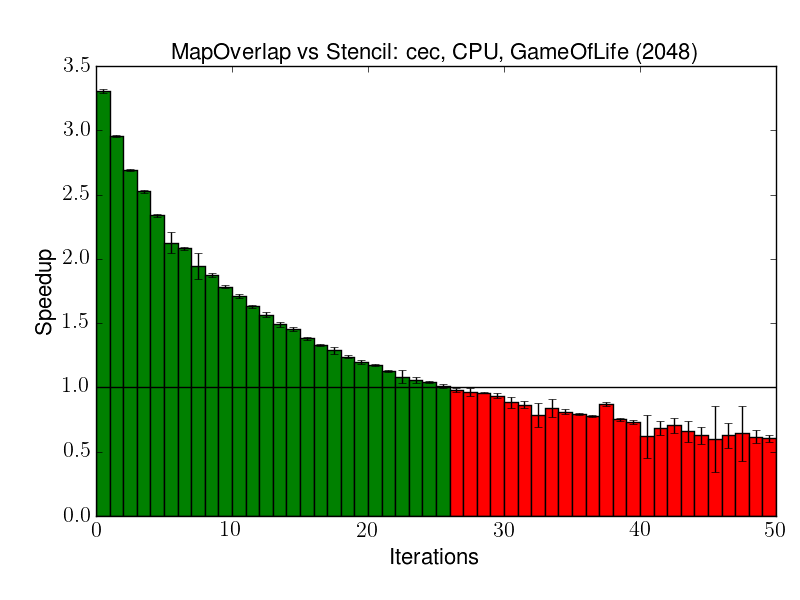
\includegraphics[width=.5\textwidth]{/home/chris/src/msc-thesis/benchmarks/results/e8/cec-CPU-GameOfLife-2048.png}
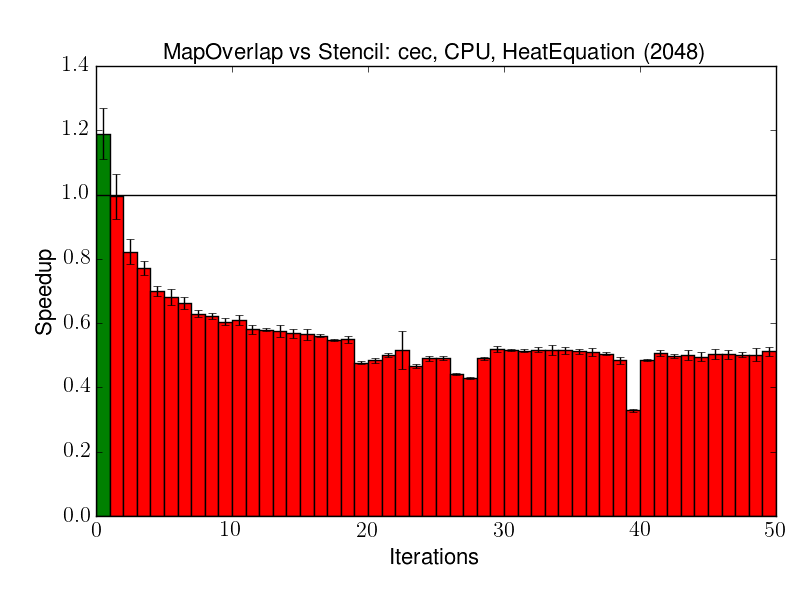
\includegraphics[width=.5\textwidth]{/home/chris/src/msc-thesis/benchmarks/results/e8/cec-CPU-HeatEquation-2048.png}
\caption{%
  Relative performance of the MapOverlap skeleton over the Stencil
  skeleton, for two different benchmarks on the same architecture.%
}
\end{figure}

\begin{figure}
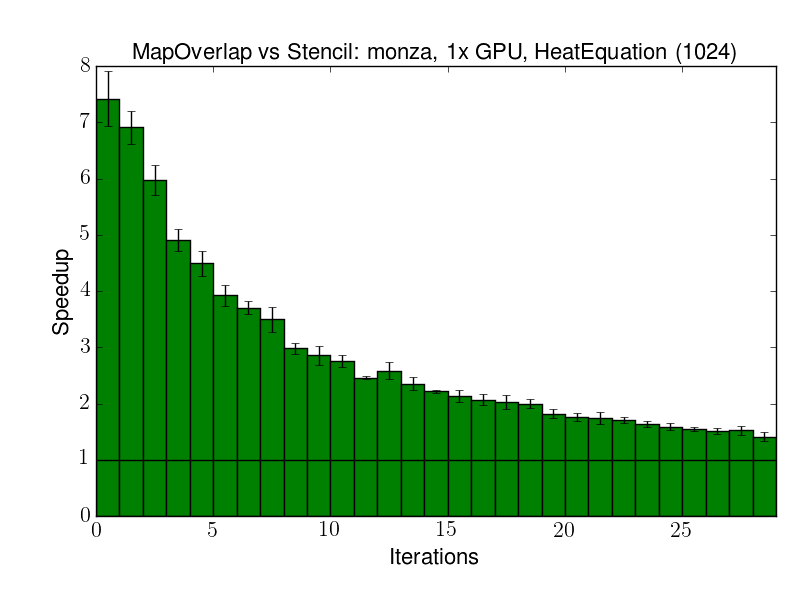
\includegraphics[width=.5\textwidth]{/home/chris/src/msc-thesis/benchmarks/results/e8/monza-1xGPU-HeatEquation-1024.png}
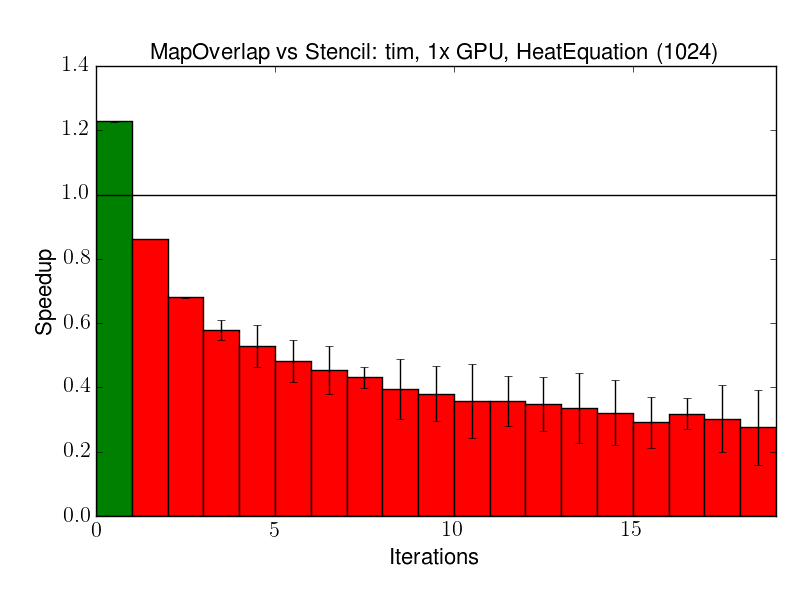
\includegraphics[width=.5\textwidth]{/home/chris/src/msc-thesis/benchmarks/results/e8/tim-1xGPU-HeatEquation-1024.png}
\caption{%
  The same program and input size for two different CP/GPU
  architectures.%
}
\end{figure}
% \begin{table}
% \footnotesize
% \centering
% \begin{tabular}{| l | l | l | l | l |}
% \hline
% \textbf{Name} & \textbf{Application} & \textbf{Skeletons used} & \textbf{Iterative?} & \textbf{LOC}\\
% \hline
% CannyEdgeDetection & Image processing & Stencil & - & 225 / 61\\
% DotProduct & Linear algebra & Zip, Reduce & - & 143 / 2\\
% FDTD & Scientific simulation & Map, Stencil & Y & 375 / 127\\
% GameOfLife & Cellular automata & Stencil & Y & 92 / 12\\
% GaussianBlur & Image processing & Stencil & - & 262 / 47\\
% HeatSimulation & Scientific simulation & Stencil & Y & 180 / 13\\
% MandelbrotSet & Fractal computation & Map & Y & 133 / 78\\
% MatrixMultiply & Linear algebra & AllPairs & - & 267 / 8\\
% SAXPY & Linear algebra & Zip & - & 149 / 3\\
% \hline
% \end{tabular}
% \caption{Benchmark applications. The LOC column shows lines of code, split between host (C++) and device (OpenCL).}
% \label{tab:benchmarks}
% \end{table}


\section{Conclusions}

Future work: ``fusing'' kernels of multi-stage iterative skeletons,
and tuning halo size for multi-GPU systems and .

Also, investigate seg faults in multi-GPU stencil computations.

\label{bibliography}
\printbibliography

\clearpage
\begin{appendices}
\section{MapOverlap vs Skeleton}\label{app:mo-vs-stencil}

Relative performance of MapOverlap vs Stencil skeletons for different
number of iterations. The ``Break-even point'' is the number of
iterations at which point the Stencil kernel is faster than
MapOverlap. With 3 GPUs on tim, and 2 GPUs on monza, one or more of
the programs runs aborted with a Segmentation Fault. No results are
provided for these configurations.

\begin{table}
\footnotesize
\centering
\begin{tabular}{| l | l | l | l | l | l |}
\hline
\textbf{Host} & \textbf{Devices} & \textbf{Application} & \textbf{Data Size} & \textbf{Speedups} & \textbf{Break-even point}\\
\hline
cec & CPU & GameOfLife & 1024 & 3.60 \ldots 1.64 1.96 \textit{0.80} & 43 \\
cec & CPU & GameOfLife & 2048 & 3.30 \ldots 1.04 1.01 \textit{0.98} & 27 \\
cec & CPU & GameOfLife & 4096 & 2.24 1.72 \textit{1.43} & > 5 \\
cec & CPU & HeatEquation & 1024 & 3.80 \ldots 1.24 1.23 \textit{1.22} & > 79 \\
cec & CPU & HeatEquation & 2048 & 3.45 \ldots 1.07 1.03 \textit{0.96} & 24 \\
cec & CPU & HeatEquation & 4096 & 2.26 1.78 \textit{1.40} & > 5 \\
whz5 & 1x GPU & GameOfLife & 4096 & 1.27 \textit{1.00} & 2 \\
whz5 & 1x GPU & HeatEquation & 4096 & 1.27 \textit{1.00} & 2 \\
tim & 1x GPU & GameOfLife & 1024 & 1.65 1.16 \textit{0.86} & 3 \\
tim & 1x GPU & GameOfLife & 2048 & 1.47 \textit{1.00} & 2 \\
tim & 1x GPU & GameOfLife & 4096 & 1.46 1.00 \textit{0.76} & 3 \\
tim & 2x GPU & GameOfLife & 1024 & 1.40 \textit{0.98} & 2 \\
tim & 2x GPU & GameOfLife & 2048 & 1.54 \textit{1.00} & 2 \\
tim & 2x GPU & GameOfLife & 4096 & 1.53 1.00 \textit{0.75} & 3 \\
tim & 3x GPU & GameOfLife & 1024 &  & - \\
tim & 3x GPU & GameOfLife & 2048 &  & - \\
tim & 3x GPU & GameOfLife & 4096 &  & - \\
tim & 4x GPU & GameOfLife & 1024 & 1.44 \textit{0.96} & 2 \\
tim & 4x GPU & GameOfLife & 2048 & 1.57 \textit{0.95} & 2 \\
tim & 4x GPU & GameOfLife & 4096 & 1.58 \textit{0.98} & 2 \\
tim & 1x GPU & HeatEquation & 1024 & 1.70 1.16 \textit{0.88} & 3 \\
tim & 1x GPU & HeatEquation & 2048 & 1.47 1.00 \textit{0.76} & 3 \\
tim & 1x GPU & HeatEquation & 4096 & 1.47 1.01 \textit{0.77} & 3 \\
tim & 2x GPU & HeatEquation & 1024 & 1.40 \textit{0.96} & 2 \\
tim & 2x GPU & HeatEquation & 2048 & 1.55 \textit{1.00} & 2 \\
tim & 2x GPU & HeatEquation & 4096 & 1.54 1.01 \textit{0.74} & 3 \\
tim & 3x GPU & HeatEquation & 1024 &  & - \\
tim & 3x GPU & HeatEquation & 2048 &  & - \\
tim & 3x GPU & HeatEquation & 4096 &  & - \\
tim & 4x GPU & HeatEquation & 1024 & 1.51 \textit{0.96} & 2 \\
tim & 4x GPU & HeatEquation & 2048 & 1.61 \textit{0.99} & 2 \\
tim & 4x GPU & HeatEquation & 4096 & 1.57 \textit{0.98} & 2 \\
monza & 1x GPU & GameOfLife & 1024 & 1.55 \ldots 1.09 1.04 \textit{0.96} & 22 \\
monza & 1x GPU & GameOfLife & 2048 & 1.49 \ldots 1.12 1.01 \textit{0.96} & 6 \\
monza & 1x GPU & GameOfLife & 4096 & 1.60 1.18 \textit{0.96} & 3 \\
monza & 2x GPU & GameOfLife & 1024 &  & - \\
monza & 2x GPU & GameOfLife & 2048 &  & - \\
monza & 2x GPU & GameOfLife & 4096 &  & - \\
monza & CPU & GameOfLife & 1024 & 1.44 \ldots 1.09 1.03 \textit{0.99} & 9 \\
monza & CPU & GameOfLife & 2048 & 1.40 1.14 \textit{0.92} & 3 \\
monza & CPU & GameOfLife & 4096 & 1.50 \textit{0.83} & 2 \\
monza & 1x GPU & HeatEquation & 1024 & 1.59 \ldots 1.13 1.11 \textit{1.11} & > 20 \\
monza & 1x GPU & HeatEquation & 2048 & 1.65 \ldots 1.12 1.03 \textit{0.96} & 6 \\
monza & 1x GPU & HeatEquation & 4096 &  & - \\
monza & 2x GPU & HeatEquation & 1024 &  & - \\
monza & 2x GPU & HeatEquation & 2048 &  & - \\
monza & 2x GPU & HeatEquation & 4096 &  & - \\
monza & CPU & HeatEquation & 1024 & 1.40 \ldots 1.05 1.03 \textit{0.99} & 10 \\
monza & CPU & HeatEquation & 2048 & 1.52 1.16 \textit{0.97} & 3 \\
monza & CPU & HeatEquation & 4096 & 1.52 \textit{0.88} & 2 \\
\hline
\end{tabular}

%\begin{tabular}{| l | l | l | l | l | l |}
\hline
\textbf{Host} & \textbf{Devices} & \textbf{Application} & \textbf{Data Size} & \textbf{Speedups} & \textbf{Break-even point}\\
\hline
cec & CPU & GameOfLife & 1024 & 3.44 \ldots 1.14 1.45 \textit{0.77} & 43 \\
cec & CPU & GameOfLife & 2048 & 2.98 \ldots 1.07 1.02 \textit{0.97} & 16 \\
cec & CPU & GameOfLife & 4096 & 1.95 1.41 1.17 \textit{0.99} & 4 \\
cec & CPU & HeatEquation & 1024 & 3.65 \ldots 1.02 1.03 \textit{1.00} & 58 \\
cec & CPU & HeatEquation & 2048 & 3.11 \ldots 1.05 1.01 \textit{0.95} & 16 \\
cec & CPU & HeatEquation & 4096 & 1.87 1.45 1.14 \textit{0.98} & 4 \\
whz5 & 1x GPU & GameOfLife & 4096 & 1.13 \textit{0.91} & 2 \\
whz5 & 1x GPU & HeatEquation & 4096 & 1.13 \textit{0.91} & 2 \\
tim & 1x GPU & GameOfLife & 1024 & 1.20 \textit{0.86} & 2 \\
tim & 1x GPU & GameOfLife & 2048 & 1.12 \textit{0.79} & 2 \\
tim & 1x GPU & GameOfLife & 4096 & 1.11 \textit{0.79} & 2 \\
tim & 2x GPU & GameOfLife & 1024 & 1.21 \textit{0.86} & 2 \\
tim & 2x GPU & GameOfLife & 2048 & 1.29 \textit{0.87} & 2 \\
tim & 2x GPU & GameOfLife & 4096 & 1.28 \textit{0.87} & 2 \\
tim & 3x GPU & GameOfLife & 1024 &  & - \\
tim & 3x GPU & GameOfLife & 2048 &  & - \\
tim & 3x GPU & GameOfLife & 4096 &  & - \\
tim & 4x GPU & GameOfLife & 1024 & 1.32 \textit{0.90} & 2 \\
tim & 4x GPU & GameOfLife & 2048 & 1.42 \textit{0.89} & 2 \\
tim & 4x GPU & GameOfLife & 4096 & 1.43 \textit{0.92} & 2 \\
tim & 1x GPU & HeatEquation & 1024 & 1.23 \textit{0.86} & 2 \\
tim & 1x GPU & HeatEquation & 2048 & 1.12 \textit{0.79} & 2 \\
tim & 1x GPU & HeatEquation & 4096 & 1.12 \textit{0.79} & 2 \\
tim & 2x GPU & HeatEquation & 1024 & 1.21 \textit{0.85} & 2 \\
tim & 2x GPU & HeatEquation & 2048 & 1.30 \textit{0.87} & 2 \\
tim & 2x GPU & HeatEquation & 4096 & 1.29 \textit{0.87} & 2 \\
tim & 3x GPU & HeatEquation & 1024 &  & - \\
tim & 3x GPU & HeatEquation & 2048 &  & - \\
tim & 3x GPU & HeatEquation & 4096 &  & - \\
tim & 4x GPU & HeatEquation & 1024 & 1.38 \textit{0.90} & 2 \\
tim & 4x GPU & HeatEquation & 2048 & 1.45 \textit{0.92} & 2 \\
tim & 4x GPU & HeatEquation & 4096 & 1.42 \textit{0.92} & 2 \\
monza & 1x GPU & GameOfLife & 1024 & 1.53 \ldots 1.05 1.04 \textit{1.00} & 21 \\
monza & 1x GPU & GameOfLife & 2048 & 1.43 \ldots 1.11 1.07 \textit{0.98} & 5 \\
monza & 1x GPU & GameOfLife & 4096 & 1.54 1.16 \textit{0.96} & 3 \\
monza & 2x GPU & GameOfLife & 1024 &  & - \\
monza & 2x GPU & GameOfLife & 2048 &  & - \\
monza & 2x GPU & GameOfLife & 4096 &  & - \\
monza & CPU & GameOfLife & 1024 & 1.39 \ldots 1.07 1.01 \textit{0.95} & 6 \\
monza & CPU & GameOfLife & 2048 & 1.23 1.03 \textit{0.89} & 3 \\
monza & CPU & GameOfLife & 4096 & 1.14 \textit{0.83} & 2 \\
monza & 1x GPU & HeatEquation & 1024 & 1.56 \ldots 1.06 1.07 \textit{0.99} & 20 \\
monza & 1x GPU & HeatEquation & 2048 & 1.57 \ldots 1.17 1.08 \textit{0.99} & 5 \\
monza & 1x GPU & HeatEquation & 4096 &  & - \\
monza & 2x GPU & HeatEquation & 1024 &  & - \\
monza & 2x GPU & HeatEquation & 2048 &  & - \\
monza & 2x GPU & HeatEquation & 4096 &  & - \\
monza & CPU & HeatEquation & 1024 & 1.35 \ldots 1.18 1.07 \textit{0.98} & 5 \\
monza & CPU & HeatEquation & 2048 & 1.31 1.03 \textit{0.88} & 3 \\
monza & CPU & HeatEquation & 4096 & 1.14 \textit{0.83} & 2 \\
\hline
\end{tabular}

\end{table}

\end{appendices}

\end{document}
